\graphicspath{{8/figures/}}
\chapter{Conclusion}
\label{chp:conclusion}

We've covered a lot of ground here.
Shed some tears, had some laughs.
But now it's time to say goodbye.
This chapter concludes this work in two parts.
First, Section \ref{sec:summary} summarizes the work performed and novel contritributions made therein.
Second, Section \ref{sec:future} offers perspectives for the future, including an assessment of outstanding challenges and the potential impact of continued research in this domain.

\section{Summary of Findings}

Automatic music description is at the heart of content-based music informatics research.
This is super useful for problems where manual annotation doesn't scale, such as acoustic similarity, as well as problems where most people lack the musical expertise to perform the task at all, such as transcription.
While the topic has real value, progress seems to have slowed, and we wanted to know why.
Thus common practice in automatic music description was revisited, leading to the identification of three deficiencies worth addressing: hand-crafted feature design is not sustainable, shallow architectures are fundamentally limited, and short-time analysis alone fails to capture long-term musical structure.
Deep architectures and feature learning demonstrate promise in music analysis tasks, thus motivating the exploration of deep learning in automatic music description.

At this point it was necessary to consider what is ``deep learning'', and why is this an option now?
The history of the field was re-examined, showing that after an over-hyped introduction, neural networks languished through the latter part of the 20th century.
This period of skepticism and disinterest gave technology time to catch up to the theory, and after a serious of significant research contributions, deep learning made a triumphant return to the fore of computer science, toppling longstanding benchmarks seemingly overnight.
While this has brought about a second wave of hype and interest, a more established theory of deep networks is being curated.
As reviewed, the modern practice of deep learning consists of a handful of modular processing blocks, strung together in differentiable functions and numerically optimized to an objective function via gradient-based methods, complemented by a growing suite of practical tricks of the trade.

Having reviewed the modern core of deep learning, this work shifted focus to explore these methods directly.
As a first inquiry, a deep convolutional network was applied to the task of timbre similarity, achieving three goals:
the model is able to learn relevant signal-level features that give rise to source identification;
the resulting output space is organized in a semantically meaningful way;
and the smoothness of the space is indicated by error analysis.
The approach presented here also offers novel extensions to previous efforts in pairwise training, achieving extremely robust representations despite a considerable reduction in dimensionality.
And perhaps most importantly, these results are obtained without the need for costly subjective pairwise ratings of content.

Whereas timbre similarity served as a relatively constrained problem, the shift to automatic chord estimation sought to test the limits of deep learning at a well-established music informatics challenge.
Competitive performance is achieved with a deep convolutional neural network, evaluated in both a conventional and large-vocabulary variant of the task.
Somewhat more interestingly, rigorous error analysis reveals that efforts in automatic chord estimation are converging to a glass ceiling, due in large part to the objective formulation of an often subjective experience.
The problems caused by the tenuous nature of ``ground truth'' annotations are exacerbated by efforts to treat chord estimation as a flat, rather than hierarchical, classification task.
Therefore, the singlemost critical advancement facing the topic of automatic chord estimation is a re-evaluation of the task the community is attempting to solve and the data used to do so.

Despite these difficulties, the chord estimation data is leveraged to ask a slightly different question: can a model be built to automatically predict chords as guitar tablature?
Using yet another deep convolutional architecture, global performance statistics are improved over the general chord estimation system, while offering significant practical benefits.
In addition to being a high-performing system, the fretboard estiamtions are immediately human-readable and thus attractive from a user experience perspective.
Such a representation is also advantageous from a data collection, correction, and validation standpoints, significantly reducing the degree of prerequisite skill necessary to contribute annotations.

Finally, the various open source software artifacts developed in the course of this research are introduced and detailed:
\texttt{jams}, the structured music annotation format designed for multiplicity of both annotator perspective and task namespace;
\texttt{biggie}, an approach to managing large collections of numerical data for training stochastic learning algorithms;
\texttt{optimus}, a user-friendly library for describing and serializing trainable processing graphs;
\texttt{mir\_eval}, a suite of evaluation tools for benchmarking music description algorithms;
and finally \texttt{dl4mir}, a common framework for the systems and results presented here.


\section{Perspectives on Future Work}
\label{sec:future}

% Bob L. Sturm: Whether or not a dataset, or set of datasets, is ``good'' depends on its relevance to the scientific question that is being asked. In a very real sense, the least of one's worries should be datasets. Much more effort must be made in the design, implementation and analysis of valid and relevant experiments.


The research cycle for computational behavioral modeling consists of six steps:

% \begin{enumerate}
% \item Define the problem.
% \item Collect data.
% \item Build a solution.
% \item Evaluate the model.
% \item Repeat.
% \end{enumerate}

\begin{enumerate}
\item Define the problem.
\item Collect data.
\item Form a hypothesis.
\item Conduct experiments to test the hypothesis.
\item Interpret and analyze the experimental results.
\item Repeat.
\end{enumerate}

This work explored deep learning as a flexible, yet powerful, answer for (3), but there is much work to be done in the other discrete stages.
We could extend the list of deficiencies to include another; methodological issues in music informatics.

% Problem formulation and rigor / definitions
Most current music informatics challenges evolved naturally from a logical progression of work.
Many research topics have inertia, and thus the problem definition is defined implicitly, rather than explicitly.
Other facets of the research cycle have or had influenced the problem definition.
Often, this was driven in no small part by the data available to a researcher.
What is it to define a problem?
You have to worry about scope, requirements, and limitations.

What is the problem chord recognition is really trying to solve?
``Can a machine provide reliable chord transcriptions?'' is a very different question from ``Can a machine predict these chord transcriptions?''
Importantly, it's not hard to imagine even a human based system that achieves a ``yes'' and ``no'' respectively.

In others formulation of the music description task is underspecified.
This is consistent with at least part of the position motivated recently by Sturm \cite{}, who argues that classic problems in music informatics lack sufficiently rigorous definitions to ever be solved.
Though not as egregious as a task like genre, this is the primary outcome from the chapter on chord recognition, showing that a lack of clarity in the task description makes the target an impossilbe one to hit.

% Data collection
% Using data you trust; garbage in, garbage out
You can train on noisy data, but you cannot and should not evaluate an algorithm objectively with it.
This is sensitive to the question being asked.

% Form and test a hypothesis
We're really good at this part.
We build a lot of stuff, so much so that we've kind of forgotten about the other things.


% Evaluation
% objective versus subjective eval
Returning to the beginning of this inquiry, it was stated that the goal of evaluation is to leverage objective measures of subjective experience, being that the true measure of value is system agreement with human experts.
But what does it mean for this goal when we find that humans don't agree with other humans?
Or perhaps







\begin{figure}
\begin{centering}
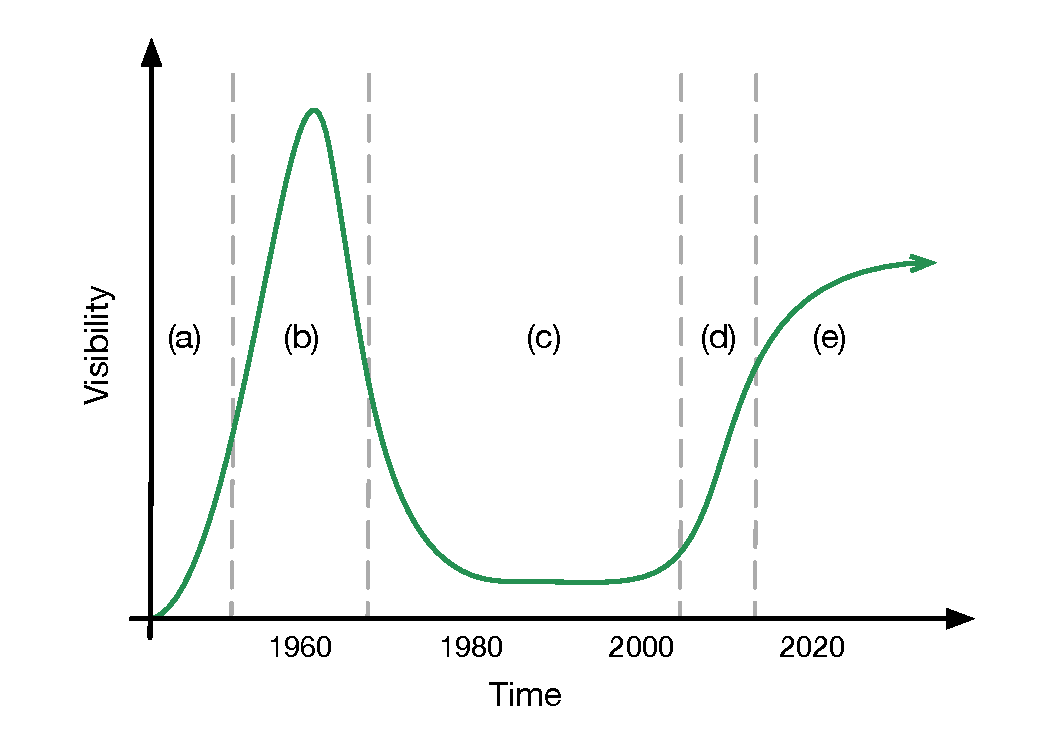
\includegraphics[width=0.6\textwidth]{deephype}
\caption{\emph{Gartner Hype cycle of neural networks.}
\label{fig:deephype}
\end{centering}
\end{figure}

% Tie it all together
Thus, after an impeccably rocky start, neural networks are finally having their day in the sun.
Shown in Figure \ref{fig:deephype}, it is interesting to consider that the path of deep learning has closely followed Gartner's technology Hype Cycle.
Settling in as another computational tool in the belt (PCA or SVMs), following the hype cycle; we are in the path to productivity.
Have a better idea of how they can work.
What have we actually learned from previous struggles? Are we at risk of repeating the past?
More domains are adopting, but not all domains have.

\subsection{Outstanding Challenges}

Reflecting on the entire discourse, there are a few legitimate obstacles to this line of research.
The most immediate hurdle facing the adaptation of deep learning to music signal processing is merely a matter of literacy and the successful application of these methods to classic problems in MIR.
There is an empirical sense of skepticism regarding neural networks among many in the various perceptual AI communities, including MIR, due in no small part to the exaggerated promises of very early research, and popular opinion has not evolved with the science.
One step toward updating this perspective is through discussions like this one, by demystifying the proverbial ``black box'' and understanding what, how, and why these methods work.
Additionally, reframing traditional problems in the viewpoint of deep learning serves as an established starting point to begin developing a good comprehension of implementing and realizing these systems.
In a similar vein, the MIR community also possesses a mastery of digital signal theory and processing techniques, insight that could, and should, be applied to deep networks to better formulate novel or alternative theoretical foundations.

Another, more widely known problem is the practical difficulty behind getting such methods to ``work,'' which takes a few different forms.
Though the features, and more specifically the parameters, learned by the model are data-driven, the successful application of deep learning necessitates a thorough understanding of these methods and how to apply them to the problem at hand.
Various design decisions, such as model selection, data pre-processing, and carefully choosing the building blocks of the system, can impact performance on a continuum from negligible differences in overall results to whether or not training can, or will, converge to anything useful.
Likewise, the same kind of intuition holds for adjusting the various hyperparameters ---learning rate, regularizers, sparsity penalties--- that may arise in the course of training.
The important thing to recognize though is that these are skills to be learned.
Using deep learning presents a design problem not altogether different from the one with which we are familiar, but the approach is overtly more abstract and conceptual, placing a greater emphasis on high-level decisions like the choice of network topology or appropriate loss function.

That said, one of the more enticing challenges facing music informatics is that time-frequency representations, though two-dimensional, are fundamentally \emph{not} images.
When considering the application of deep learning to MIR problems, it is prudent to recognize that the majority of progress has occurred in computer vision.
While this gives our community an excellent starting point, there are many assumptions inherent to image processing that start to break down when working with audio signals.
One such instance is the use of local receptive fields in deep learning, common in CNNs and, more recently, tiled networks \cite{Le2010}.
In these architectures, it is known that the strongest correlations in an image occur within local neighborhoods, and this knowledge is reflected in the architectural design.
Local neighborhoods in frequency do not share the same relationship, so the natural question becomes, ``what architectures \emph{do} make sense for time-frequency representations?''
As we saw previously, CNNs yield encouraging results on time-frequency representations of audio, but there are certainly better models to be discovered.
This is but one open question facing deep learning in music signal processing, and a concerted research effort will likely reveal more.


\subsection{Potential Impact}

In addition to hopefully advancing the discipline beyond current glass ceilings, there are several potential benefits to the adoption and research of deep learning in music informatics.
Though learning can discover useful features that were previously overlooked or not considered, this advantage is amplified for new challenges and applications that do not offer much guiding intuition.
For tasks like artist identification or automatic mixing, it is difficult to comprehend, much less articulate, exactly what signal attributes are informative to the task and how an implementation might robustly capture this information.
These problems can, however, be quantified by an objective function ---these songs are by the same artist, or this is a better mix than that one--- which allows for an automated exploration of the solution space.
In turn, such approaches may subsequently provide insight into the latent features that inform musical judgements, or even lead to deployable systems that could adapt to the nuances of an individual.

Deep learning also offers practical advantages toward accelerating research.
Rather than trying to compare the instances from one class of functions, evaluation can take place at the class level.
This process has the potential to be significantly faster than current research approaches because numerical methods attempt to automatically optimize the same objective function we do by hand.
Additionally, unsupervised learning is able to make use of all recorded sound, and the data-driven prior that it leverages can be steered by creating specific distributions, e.g., learn separate priors for rock versus jazz.
Finally, music signals provide an interesting setting in which to further explore the role of \emph{time} in perceptual AI systems, and has the potential to influence other time-series domains like video or motion capture data.
